\documentclass[11pt,a4paper]{article}

\usepackage[utf8]{inputenc}
\usepackage[T1]{fontenc}
\usepackage{lmodern}
\usepackage[margin=2.5cm]{geometry}
\usepackage{amsmath,amssymb}
\usepackage{graphicx}
\usepackage{booktabs}
\usepackage{array}
\usepackage[table]{xcolor}
\usepackage{pdflscape}
\usepackage{afterpage}
\usepackage{tikz}
\usetikzlibrary{arrows.meta,decorations.pathreplacing,patterns}
\usepackage{siunitx}
\usepackage[hidelinks]{hyperref}

\graphicspath{{figures/}}

\title{Early embryo differentiation in zebrafish}
\author{Samuel Pastva}
\date{\today}

\newcommand{\citationneeded}{[\emph{citation needed}]}

\begin{document}

\maketitle

\section{Glossary and preliminaries}

Because biology likes to use big, fancy words, we first have to build a glossary of terms that will appear in this report. Most are relatively ``standard'' in the literature, but many have slightly different meaning across subfields, so this section can be also viewed as term definitions.

\begin{itemize}
	\item A \textbf{transcription factor (TF)} is a protein that directly influences the transcription process, either by participating in it, or by modifying the environment that influences the actual transcription machinery (e.g., opening or closing chromatin). Note that this is intentionally broader than the strict textbook definition, which only covers proteins that bind specific DNA sequences; here, we also include co-factors and chromatin remodelers.
	\item Time points in zebrafish embryo development are usually denoted in \textbf{hours post fertilization (hpf)}. We will shorten this to \textbf{hours (h)} when clear from context. We will be mostly interested in the development processes taking place until approx. \textbf{12hpf}.
	\item Since zebrafish are simple organisms, the embryo development is also relatively stable and easy to reproduce. The most important environmental factor is \textbf{temperature}, which is typically \textbf{28.5 °C}. Other temperatures within acceptable rates should have roughly linear influence on the development speed \citationneeded. Other factors like pH, medium density or oxygen levels also impact development, but the embryo is robust to small, reasonable variations in them \citationneeded.
	\item An embryo cell can be \textbf{totipotent}, \textbf{pluripotent}, or \textbf{multipotent}. Totipotent means it can differentiate into internal embryo cells, or external cell layers enveloping the embryo (\textbf{extra-embryonic cells}). Pluripotent means it can differentiate into any embryo cell, but not into an extra-embryonic cell. Multipotent means the cell can differentiate within a specific lineage (e.g., endoderm), but not outside of that specific lineage (at least not without a significant intervention).
	\item We can also distinguish cells by how \emph{robustly} they are differentiated so far. Note that these terms are originally defined based on what happens to the cell across various environments, not necessarily by the epigenetics and transcriptome, so we are ``extrapolating'' a bit here to what is causing these terms to be well defined in the first place.
	\begin{itemize}
		\item A cell is \textbf{primed} if its epigenetics admit a particular differentiation event (relevant chromatin is open, important TF is expressed but not causing transcription yet, etc.). A cell can be primed towards many lineages at the same time. Importantly, a primed cell will not differentiate without some additional ``signal'' triggering the differentiation.
		\item A cell is \textbf{specified} if it is actively transcribing RNA of a particular cell type, and will continue this process in a neutral environment. In other words, the transcription has been started and is somewhat self-sustaining, but can be easily disrupted by an unexpected ``signal''.
		\item A cell is \textbf{determined} if it is specified, but it can maintain its own identity when encountering an opposing, but reasonable ``signal'' (i.e., a signal that would naturally occur somewhere in the organism). Determination can be driven by a stronger self-sustaining GRN feedback loop, as well as by epigenetic changes.
		\item A cell is \textbf{differentiated} if it is determined, and it has undergone morphological changes associated with its cell type, including additional epigenetic changes to further increase robustness against signaling perturbations.
		\item The expression profile of a specified / determined / differentiated cell can be different, despite being ``the same cell type''. The cell is actively producing TFs that will lead to epigenetic changes required for determination / differentiation, but this transcription can eventually turn off once the cell is ``sufficiently committed''.
		\item The process is hierarchical (cell type A differentiates into B, which turns into C, \dots), and for the intermediate cell types, the cell does not have to pass all stages. For example, pluripotent cells will never be truly differentiated, or even determined. Similarly, stages can interleave across cell types, so a cell can be determined type A, but specified type B, and primed type C, meaning it will maintain identity A on its own, is already developing expression profile of type B, and is able to eventually become type C if a signal is given.
	\end{itemize}

	\item A zebrafish embryo goes through several ``high-level'' developmental stages: \textbf{zygote (0-0.75h)}, \textbf{cleavage (0.75-2.25h)}, \textbf{blastula (2.25-5.25h)}, and \textbf{gastrula (5.25-10h)}.
	\begin{itemize}
		\item In the zygote and cleavage stage, the embryo looks mostly uniform. However, it is not fully symmetric: some maternal factors (dorsal determinants, germ plasm) are already localized asymmetrically (see MBT below).
		\item During blastula, the surface layer of extra-embryonic cells is starting to split off. These are the \textbf{enveloping layer} (EVL) and \textbf{yolk syncytial layer} (YSL); one guards the embryo from the environment, and one is an interface with the yolk on which the embryo rests. Remaining cells are also called \textbf{deep cells}.
		\item A \textbf{midblastula transition (MBT)} occurs around \textbf{2.75hpf}. Until that point, the cells are predominantly driven by the maternal transcriptome present in the zygote (a small first wave of zygotic transcription already starts around the 64-cell stage). Until MBT, the whole cell population is essentially synchronous. Nevertheless, several important decisions are already made in this period, driven by maternal factors:
		\begin{itemize}
			\item formation of the YSL and EVL (YSL forms at 512-1024 cells; Figure~\ref{fig:development});
			\item specification of a small group of \textbf{primordial germ cells}, which inherit maternal \textbf{germ plasm} during cleavage;
			\item the \textbf{dorsal-ventral} axis (see below), determined by maternal dorsal determinants that are transported to one side of the embryo.
		\end{itemize}
		\emph{The causes of these decisions mostly can't be observed through RNA expression} (only the consequences), since they rely on localization of maternal proteins. Also, \emph{the overall mass of the embryo does not change much} during blastula and gastrula (the cells mostly thin out and spread); actual growth comes later. After MBT, the cells divide asynchronously, hence there is no longer a clear cell doubling pattern.
		\item During gastrula, the embryo splits along the \emph{radial axis} (the deep--superficial direction, perpendicular to the embryo surface; not to be confused with the radial symmetry of the blastula around the animal-vegetal axis) into \textbf{hypoblast} (develops into \textbf{mesendoderm}) and \textbf{epiblast} (develops into \textbf{ectoderm}). Note that hypoblast and epiblast are purely positional terms: Both are part of the \textbf{germ ring}, with hypoblast being the inner layer (adjacent to the yolk), while epiblast is the outer layer (see also Figure~\ref{fig:development}). In other words, a cell can be a part of hypoblast and of mesendoderm; one is the location, the other is the expression profile. The germ ring is the \textbf{margin} of the embryo (you can see cells called ``marginal'', meaning they belong to this region). The process of separation into hypoblast/epiblast along the germ ring is called \textbf{internalization}. During gastrula, the epiblast still contains mesendoderm precursors that internalize later; only once internalization finishes does epiblast fully correspond to ectoderm. 
		\item Within the gastrula phase, the embryo also visibly splits along the \textbf{dorsal-ventral} axis (dorsal is back / spine, ventral is front / belly). This split is marked by a \textbf{shield} formation on the dorsal side of the embryo. Note that the dorsal side itself is determined much earlier (maternally, see MBT above); the shield is where it first becomes morphologically visible. This is again mostly a positional term (i.e., shield is not an expression profile). However, cells in the shield do produce various signaling molecules that reinforce the dorsal-ventral split, and later also the anterior-posterior separation (see below). Sometimes, they are called \textbf{organizer cells}.
		\item The term \textbf{lateral} (and its opposite, \textbf{medial}) is used in two related senses. During gastrula, it refers to position along the margin: viewed from the animal pole, the margin is a circle with the dorsal side (shield) on one end and the ventral side on the opposite end; the \emph{lateral} margin are the two sides in between (left and right). In the body, it refers to the distance from the midline (the future spine): \emph{medial} is close to the midline, \emph{lateral} is far from it. The two are connected, because during gastrula the cells converge towards the dorsal side, which becomes the midline of the body. A related term is \textbf{paraxial}, meaning directly alongside the midline (i.e., the body axis).
		\item After gastrula, the embryo undergoes \textbf{early segmentation}, where the split along the \textbf{anterior-posterior} (A-P) axis becomes morphologically visible (as with the other axes, A-P patterning, e.g., of the neural plate, already starts during gastrula). The A-P axis is often confused with the \textbf{animal-vegetal} axis, but these are different axes: animal-vegetal is the axis of the egg (animal pole = top, where the blastoderm sits; vegetal pole = bottom of the yolk), while A-P is the body axis, which only forms during gastrula. They are only roughly aligned (the animal region gives rise to anterior head structures, while the tail bud forms near the vegetal pole). In Figure~\ref{fig:development}, AP/VP mark the animal/vegetal pole, while Ant./Pos. mark anterior/posterior. Segmentation is beyond the scope of this document.
	\end{itemize}
	
	\item During blastula and gastrula, the embryo also undergoes \textbf{epiboly}, during which it envelops the connected yolk. This is again largely used as a timing / position marker, with Figure~\ref{fig:development} showing the individual stages. Note that the formation of a hypoblast and epiblast, as well as of a germ ring and shield are happening relatively quickly between 50\% and 60\% epiboly, but this is a morphological change; transcriptomic and epigenetic changes leading up to the formation are already happening sooner.
	
	\item Another note is that in terms of morphology and transcriptome, epiblast is essentially just the continuation of the existing deep cells, without major changes at the moment of separation. It is the hypoblast that represents a new lineage that is splitting off of epiblast in the marginal region. However, later during gastrula, the ectoderm itself splits into \textbf{neural} and \textbf{non-neural} ectoderm (the latter becoming the \textbf{epidermis}), driven by a signaling gradient along the dorsal-ventral axis, and this split is visible in the transcriptome.
\end{itemize}

\begin{figure}
	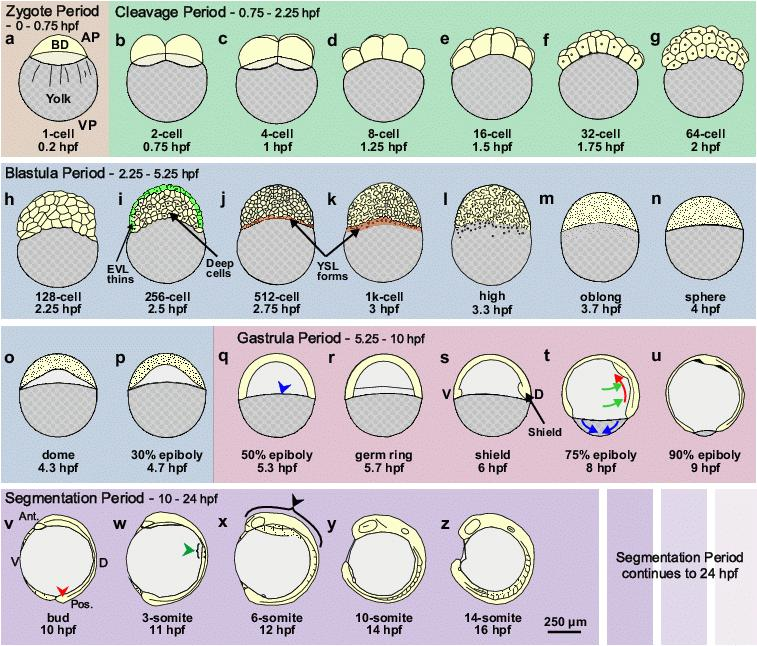
\includegraphics[width=1.0\linewidth]{figures/development.jpg}
	\caption{\url{https://www.aups.org.au/Proceedings/38/43-51/}}
	\label{fig:development}
\end{figure}

\section{Transcriptomic and epigenetic timeline}

In the previous section, we described the important terms and formations which appear during embryo development. However, these are mostly \emph{morphological} terms dictating what the embryo looks like or what is happening externally. They do not capture how the cells are evolving internally, which typically precedes morphological changes quite a bit. Also, as we discussed, these do not map directly to any meaningful definition of ``cell types'' (i.e., a ``shield cell'' is not a well defined cell type). In this section, we thus summarize the \emph{expression programs} that we expect to observe in the transcriptome during the first 12 hours, roughly when they emerge or diminish, what they do, and which earlier program they develop from. A few general remarks:

\begin{itemize}
	\item All time ranges are approximate. They denote when a program should become \emph{distinguishable in the transcriptome}, which usually precedes the corresponding morphological change by an hour or more. Also, the transitions are gradual: a new program typically first appears as a weak, graded bias within its parent population, and only later becomes a clearly separated cluster.
	\item Programs rarely ``end''; most of them keep splitting into more specific sub-programs. When we say a program diminishes, we mean it is no longer a meaningful description of the cells, because they have been replaced by its more specific descendants.
	\item Not everything is equally visible in single-cell data. Some programs are not captured at all (e.g., the YSL, which is a syncytium, not a set of cells), or involve only a handful of cells (e.g., germ cells), and the GSE106587 atlas only starts at 3.3hpf, i.e., after MBT.
\end{itemize}

Table~\ref{tab:programs} gives an overview, and Figure~\ref{fig:programs} shows the same programs as a timeline, highlighting the branching points and the spatial axis along which each split happens. The individual programs are described in more detail below.

\begin{figure}[p]
	\centering
	% Timeline of expected expression programs (see Table~\ref{tab:programs}).
% Coordinates: x = hours post fertilization, y = lane index (growing downwards).
% Requires: tikz with arrows.meta, decorations.pathreplacing and patterns.
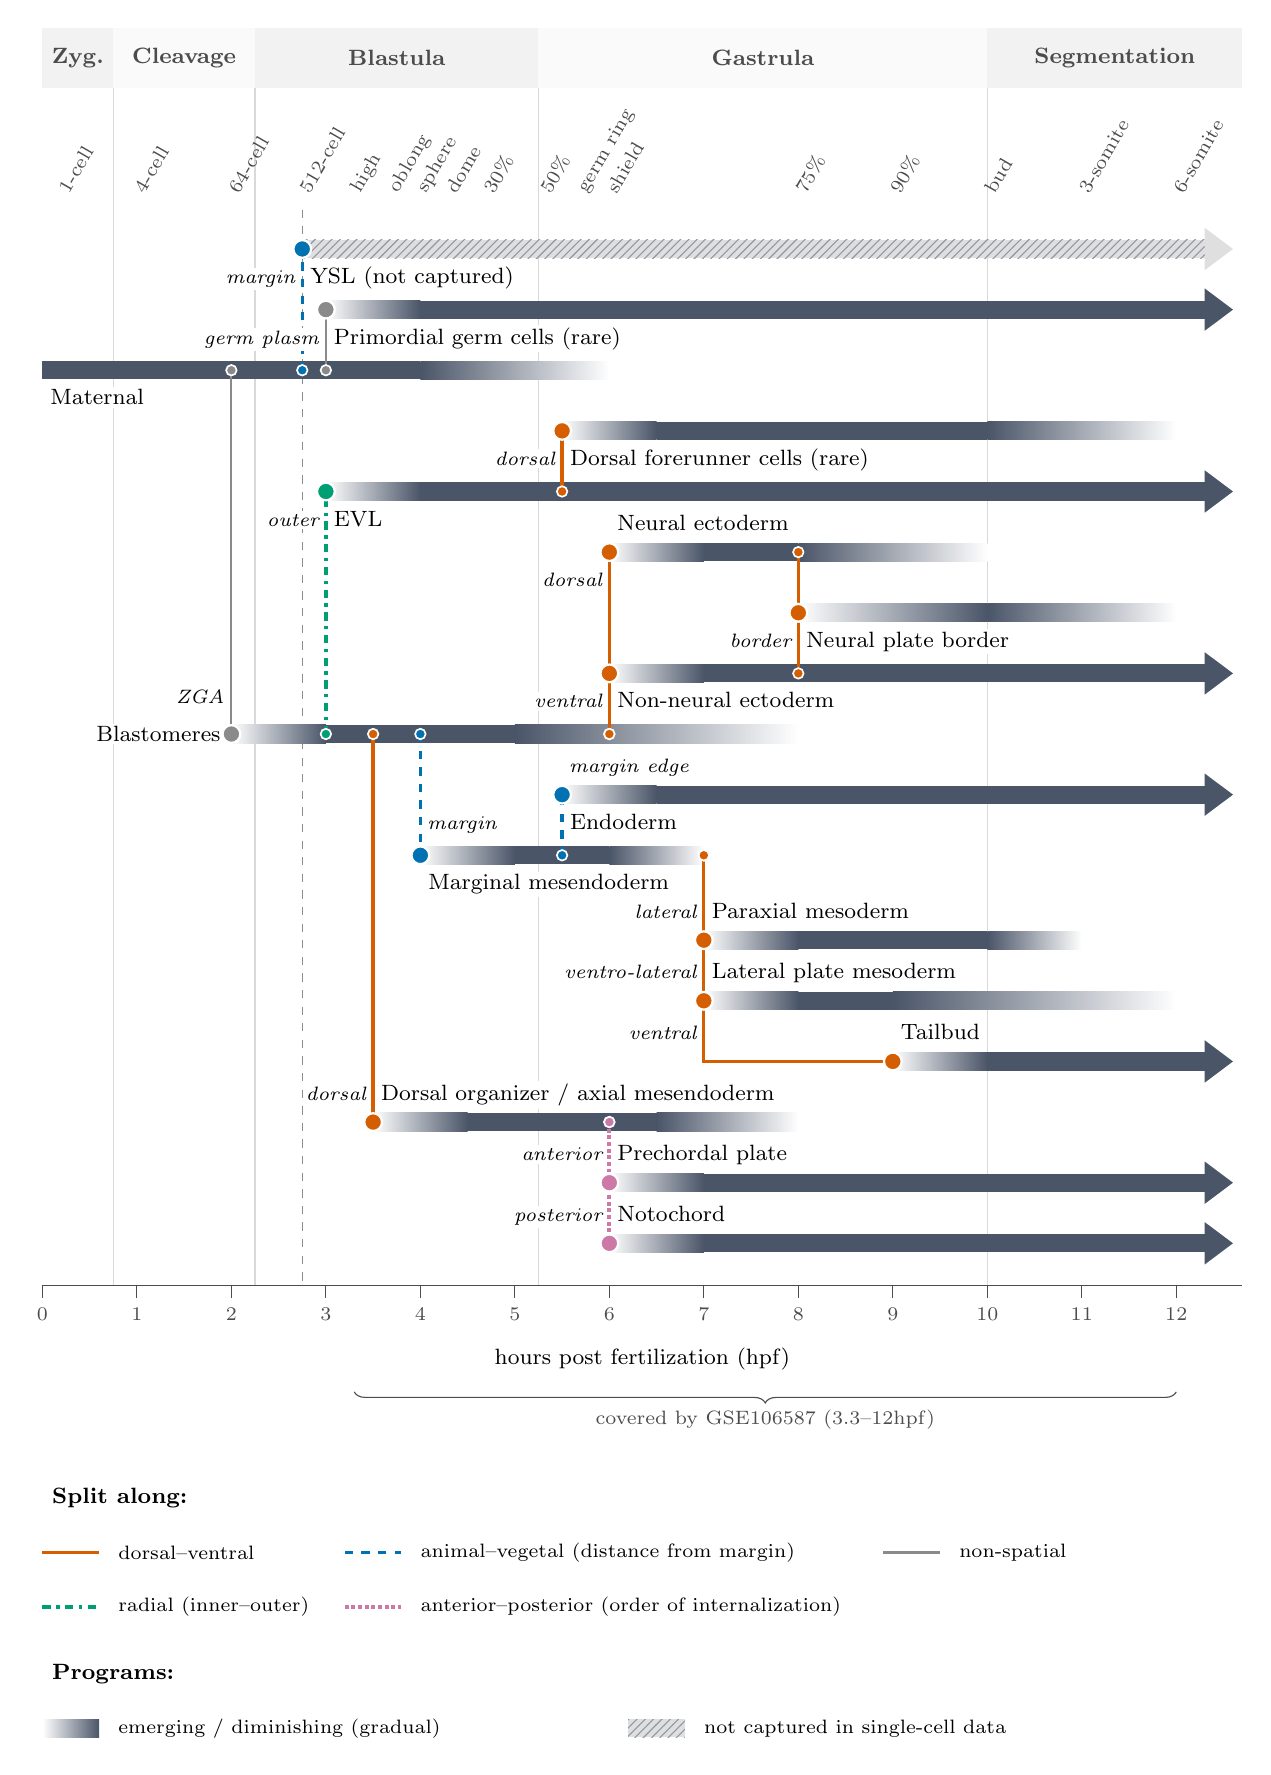
\begin{tikzpicture}[x=1.2cm, y=-0.77cm, font=\footnotesize]

	% Colors: bars are neutral, connectors encode the axis of the split.
	\definecolor{barc}{HTML}{4A5568}
	\definecolor{axdv}{HTML}{D55E00}
	\definecolor{axav}{HTML}{0072B2}
	\definecolor{axrad}{HTML}{009E73}
	\definecolor{axap}{HTML}{CC79A7}
	\definecolor{axns}{HTML}{8A8A8A}
	\tikzset{
		dv/.style={axdv, line width=1.2pt},
		av/.style={axav, line width=1.2pt, dashed},
		rad/.style={axrad, line width=1.2pt, dash dot},
		ap/.style={axap, line width=1.4pt, densely dotted},
		ns/.style={axns, line width=0.8pt},
		cond/.style={font=\scriptsize\itshape, fill=white, inner sep=1pt, anchor=base east},
		pname/.style={font=\fontsize{8.5}{10}\selectfont, fill=white, inner sep=1pt, anchor=base west},
	}

	% Baselines of labels above / below a bar (in lanes, relative to its centre).
	% Names and condition labels share them, so neighbouring labels align.
	\def\abovey{-0.36}
	\def\belowy{0.57}

	% Program names go above the bar by default, or below it after \namebelowtrue
	% (used where connectors leave the bar upwards, so they don't cross the name).
	\newif\ifnamebelow
	\newcommand{\progname}[3]{
		\ifnamebelow
			\node[pname] at (#2+0.05,#1+\belowy) {#3};
		\else
			\node[pname] at (#2+0.05,#1+\abovey) {#3};
		\fi
	}
	% \progfade{lane}{a}{b}{c}{d}{name}: emerges over [a,b], diminishes over [c,d].
	\newcommand{\progfade}[6]{
		\shade[left color=white, right color=barc] (#2,#1-0.15) rectangle (#3,#1+0.15);
		\fill[barc] (#3,#1-0.15) rectangle (#4,#1+0.15);
		\shade[left color=barc, right color=white] (#4,#1-0.15) rectangle (#5,#1+0.15);
		\progname{#1}{#2}{#6}
	}
	% \progpersist{lane}{a}{b}{name}: emerges over [a,b], persists beyond 12hpf.
	\newcommand{\progpersist}[4]{
		\shade[left color=white, right color=barc] (#2,#1-0.15) rectangle (#3,#1+0.15);
		\fill[barc] (#3,#1-0.15) rectangle (12.3,#1+0.15);
		\fill[barc] (12.3,#1-0.35) -- (12.6,#1) -- (12.3,#1+0.35) -- cycle;
		\progname{#1}{#2}{#4}
	}
	% \conn{style}{x}{parent lane}{child lane}{child start}{condition}
	% The condition label sits on the side from which the connector arrives.
	% Connectors are drawn on top of the bars: \conn only collects the lines,
	% condition labels and dots, which are then drawn (in this order) after
	% all programs. \addlabel collects a manually placed condition label.
	\def\connlines{}
	\def\connlabels{}
	\def\conndots{}
	\newcommand{\appendto}[2]{\expandafter\def\expandafter#1\expandafter{#1#2}}
	\newcommand{\addlabel}[1]{\appendto\connlabels{#1}}
	\newcommand{\conn}[6]{
		\appendto\connlines{\draw[#1] (#2,#3) -- (#2,#4) -- (#5,#4);}
		\appendto\conndots{
			\filldraw[#1, solid, draw=white, line width=0.6pt] (#2,#3) circle (1.9pt);
			\filldraw[#1, solid, draw=white, line width=0.8pt] (#5,#4) circle (3.2pt);}
		\pgfmathsetmacro{\condx}{#2-0.04}
		\pgfmathsetmacro{\condy}{#4 + (#3 > #4 ? \belowy : \abovey)}
		\edef\condtmp{\noexpand\addlabel{\noexpand\node[cond] at (\condx,\condy) {\unexpanded{#6}};}}
		\condtmp
	}

	% --- Background: developmental periods and stages -----------------------
	% Periods are shaded only in the header; thin dividers run through the plot.
	\foreach \a/\b/\name/\sh in {0/0.75/Zyg./10, 0.75/2.25/Cleavage/4, 2.25/5.25/Blastula/10, 5.25/10/Gastrula/4, 10/12.7/Segmentation/10} {
		\fill[gray!\sh] (\a,-2.65) rectangle (\b,-1.65);
		\node[font=\footnotesize\bfseries, text=black!70] at ({(\a+\b)/2},-2.15) {\name};
	}
	\foreach \t in {0.75, 2.25, 5.25, 10} {
		\draw[black!15] (\t,-1.65) -- (\t,18.1);
	}
	\foreach \t/\stage in {0.2/1-cell, 1/4-cell, 2/64-cell, 2.75/512-cell, 3.3/high, 3.7/oblong, 4/sphere, 4.3/dome, 4.7/30\%, 5.3/50\%, 5.7/germ ring, 6/shield, 8/75\%, 9/90\%, 10/bud, 11/3-somite, 12/6-somite} {
		\node[font=\scriptsize, text=black!70, anchor=west, rotate=60, inner sep=1pt] at (\t,0.1) {\stage};
	}
	\draw[black!45, dashed] (2.75,0.35) -- (2.75,18.1);

	% --- Connectors (drawn first, so bars and labels sit on top) ------------
	% Rows are ordered "middle-out": blastomeres in the middle, ectoderm and
	% extra-embryonic programs above, mesendoderm and axial programs below.
	% There is a small extra gap between the marginal mesendoderm and its
	% mesodermal descendants, to make room for the condition labels.
	\conn{ns}{2}{3}{9}{2}{}
	\addlabel{\node[cond] at (1.96,9-0.5) {ZGA};}
	\conn{av}{2.75}{3}{1}{2.75}{margin}
	\conn{ns}{3}{3}{2}{3}{germ plasm}
	\conn{dv}{6}{9}{8}{6}{ventral}
	\conn{dv}{6}{9}{6}{6}{dorsal}
	\conn{dv}{8}{8}{7}{8}{}
	\conn{dv}{8}{6}{7}{8}{}
	\addlabel{\node[cond] at (7.96,7+\belowy) {border};}
	\conn{rad}{3}{9}{5}{3}{outer}
	\conn{dv}{5.5}{5}{4}{5.5}{dorsal}
	\conn{dv}{3.5}{9}{15.4}{3.5}{dorsal}
	\conn{ap}{6}{15.4}{16.4}{6}{anterior}
	\conn{ap}{6}{15.4}{17.4}{6}{posterior}
	\conn{av}{4}{9}{11}{4}{}
	% Right of the line, so it does not cover the dorsal organizer connector.
	\addlabel{\node[cond, anchor=base west] at (4.04,10+\belowy) {margin};}
	\conn{av}{5.5}{11}{10}{5.5}{}
	\addlabel{\node[cond, anchor=base west] at (5.54,10+\abovey) {margin edge};}
	\conn{dv}{7}{11}{12.4}{7}{lateral}
	\conn{dv}{7}{11}{13.4}{7}{ventro-lateral}
	\conn{dv}{7}{11}{14.4}{9}{ventral}

	% --- Programs ------------------------------------------------------------
	\namebelowtrue
	% YSL: a syncytium, not captured in single-cell data (light, hatched).
	\fill[gray!25] (2.75,1-0.15) rectangle (12.3,1+0.15);
	\fill[gray!25] (12.3,1-0.35) -- (12.6,1) -- (12.3,1+0.35) -- cycle;
	\fill[pattern=north east lines, pattern color=barc!60] (2.75,1-0.15) rectangle (12.3,1+0.15);
	\progname{1}{2.75}{YSL (not captured)}
	\progpersist{2}{3}{4}{Primordial germ cells (rare)}
	% Maternal: present from fertilization, cleared after MBT.
	\fill[barc] (0,3-0.15) rectangle (4,3+0.15);
	\shade[left color=barc, right color=white] (4,3-0.15) rectangle (6,3+0.15);
	\progname{3}{0}{Maternal}
	\progfade{4}{5.5}{6.5}{10}{12}{Dorsal forerunner cells (rare)}
	\progpersist{5}{3}{4}{EVL}
	% Neural ectoderm branches downwards, so its name goes above the bar.
	\namebelowfalse
	\progfade{6}{6}{7}{8}{10}{Neural ectoderm}
	\namebelowtrue
	\progfade{7}{8}{10}{10}{12}{Neural plate border}
	\progpersist{8}{6}{7}{Non-neural ectoderm}
	% Blastomeres have connectors on both sides, so the name goes to the left.
	\shade[left color=white, right color=barc] (2,9-0.15) rectangle (3,9+0.15);
	\fill[barc] (3,9-0.15) rectangle (5,9+0.15);
	\shade[left color=barc, right color=white] (5,9-0.15) rectangle (8,9+0.15);
	\node[pname, anchor=east] at (1.92,9) {Blastomeres};
	\progpersist{10}{5.5}{6.5}{Endoderm}
	\progfade{11}{4}{5}{6}{7}{Marginal mesendoderm}
	\namebelowfalse
	\progfade{12.4}{7}{8}{10}{11}{Paraxial mesoderm}
	\progfade{13.4}{7}{8}{9}{12}{Lateral plate mesoderm}
	\progpersist{14.4}{9}{10}{Tailbud}
	\progfade{15.4}{3.5}{4.5}{6.5}{8}{Dorsal organizer / axial mesendoderm}
	\progpersist{16.4}{6}{7}{Prechordal plate}
	\progpersist{17.4}{6}{7}{Notochord}

	% Connectors, on top of the bars.
	\connlines
	\connlabels
	\conndots

	% --- Time axis and atlas coverage ----------------------------------------
	\draw[black!70] (0,18.1) -- (12.7,18.1);
	\foreach \t in {0,...,12} {
		\draw[black!70] (\t,18.1) -- (\t,18.3) node[below, font=\scriptsize] {\t};
	}
	\node[font=\footnotesize] at (6.35,19.3) {hours post fertilization (hpf)};
	\draw[decorate, decoration={brace, amplitude=4pt}, black!70] (12,19.85) -- (3.3,19.85)
		node[midway, below=3pt, font=\scriptsize] {covered by GSE106587 (3.3--12hpf)};

	% --- Legend ----------------------------------------------------------------
	\begin{scope}[shift={(0,21.6)}]
		\node[anchor=west, font=\footnotesize\bfseries] at (0,0) {Split along:};
		\foreach \sty/\lbl/\col/\row in {dv/dorsal--ventral/0/0.9, av/animal--vegetal (distance from margin)/3.2/0.9, ns/non-spatial/8.9/0.9, rad/radial (inner--outer)/0/1.8, ap/anterior--posterior (order of internalization)/3.2/1.8} {
			\draw[\sty] (\col,\row) -- (\col+0.6,\row);
			\node[anchor=west, font=\scriptsize] at (\col+0.7,\row) {\lbl};
		}
		\node[anchor=west, font=\footnotesize\bfseries] at (0,2.9) {Programs:};
		\shade[left color=white, right color=barc] (0,3.65) rectangle (0.6,3.95);
		\node[anchor=west, font=\scriptsize] at (0.7,3.8) {emerging / diminishing (gradual)};
		\fill[gray!25] (6.2,3.65) rectangle (6.8,3.95);
		\fill[pattern=north east lines, pattern color=barc!60] (6.2,3.65) rectangle (6.8,3.95);
		\node[anchor=west, font=\scriptsize] at (6.9,3.8) {not captured in single-cell data};
	\end{scope}
\end{tikzpicture}

	\caption{Timeline of the expected expression programs (Table~\ref{tab:programs}). Each bar is one program; shaded ends mark the (approximate) intervals in which it emerges or diminishes. The dashed vertical line marks the MBT.}
	\label{fig:programs}
\end{figure}

\afterpage{
\newgeometry{margin=2cm}
\begin{landscape}
\begin{table}
	\centering
	\small
	\setlength{\tabcolsep}{5pt}
	\renewcommand{\arraystretch}{1.25}
	\rowcolors{2}{gray!10}{white}
	\begin{tabular}{>{\raggedright\arraybackslash}p{3.9cm}>{\raggedright\arraybackslash}p{1.5cm}>{\raggedright\arraybackslash}p{1.7cm}>{\raggedright\arraybackslash}p{3.4cm}>{\raggedright\arraybackslash}p{6.0cm}>{\raggedright\arraybackslash}p{7.1cm}}
		\toprule
		Program & Emerges (hpf) & Diminishes (hpf) & Develops from & Conditions & Note \\
		\midrule
		Maternal & 0 & 4-6 & --- & deposited in the egg & actively degraded after MBT \\
		Blastomeres & 2-3 & 5-8 & maternal & zygotic genome activation (MBT) & replaced by germ layer programs; persists longest in the epiblast \\
		YSL & 2.75-3 & --- & maternal & marginal blastomeres fusing with the yolk & syncytium; not captured in single-cell data \\
		EVL & 3-4 & --- & blastomeres & outermost cell layer & becomes periderm \\
		Primordial germ cells & 3-4 & --- & maternal & inherited germ plasm & rare (a handful of cells) \\
		Dorsal organizer & 3.5-4.5 & 6.5-8 & blastomeres & dorsal margin; maternal dorsal determinants & morphologically the shield (6hpf); splits into prechordal plate and notochord \\
		Marginal mesendoderm & 4-5 & 6-7 & blastomeres & margin; signaling from YSL & forms the hypoblast; splits into endoderm and mesoderm programs \\
		Endoderm & 5.5-6.5 & --- & marginal mesendoderm & closest to the margin; strongest signaling & few cells at this stage; gut, liver, pancreas, pharynx \\
		Dorsal forerunner cells & 5.5-6.5 & 10-12 & EVL & dorsal margin, ahead of the shield & rare; form the Kupffer's vesicle \\
		Prechordal plate & 6-7 & --- & dorsal organizer & first internalized cells & anterior part becomes the hatching gland (10-12hpf) \\
		Notochord & 6-7 & --- & dorsal organizer & later internalized cells &  \\
		Paraxial mesoderm & 7-8 & 10 & marginal mesendoderm & lateral margin; further from the margin edge & splits into adaxial cells and presomitic mesoderm; segments into somites \\
		Lateral plate mesoderm & 7-8 & 9-12 & marginal mesendoderm & ventral and lateral margin & splits into heart, blood, endothelial and kidney precursors \\
		Non-neural ectoderm & 6-7 & --- & blastomeres & ventral epiblast; ventralizing signaling & becomes epidermis \\
		Neural ectoderm & 6-7 & 8-10 & blastomeres & dorsal epiblast; protected by the dorsal organizer & subdivides along the A-P axis (forebrain, midbrain, hindbrain, spinal cord) \\
		Neural plate border & 8-10 & 10-12 & neural and non-neural ectoderm & boundary between the two; intermediate signaling & splits into neural crest and placodes \\
		Tailbud & 9-10 & --- & marginal mesendoderm & ventral margin converging at the vegetal pole & includes overlying epiblast; neuromesodermal progenitors \\
		\bottomrule
	\end{tabular}
	\caption{Overview of expected expression programs. Times are approximate and refer to when the program becomes distinguishable in the transcriptome; --- means the program persists beyond 12hpf. \emph{Develops from} is always a preceding program in the table; \emph{conditions} describe where (location) or how (signaling, inheritance) the new program arises within it.}
	\label{tab:programs}
\end{table}
\end{landscape}
\restoregeometry
}

\subsection{Cleavage and blastula (0-5.25hpf)}

\begin{itemize}
	\item \textbf{Maternal program} (0hpf, cleared by approx. 4-6hpf). Transcripts deposited in the egg by the mother. They drive the cleavage divisions and activate the zygotic genome. After MBT, a large fraction of maternal transcripts is actively degraded; by the start of gastrula, the transcriptome is dominated by zygotic expression \citationneeded. In the atlas, the earliest stages (high, oblong) should show a strong maternal component shared by all cells.
	\item \textbf{Blastomeres} (approx. 2-3hpf, diminishing 5-8hpf). The ``default'' program of deep cells after zygotic genome activation (ZGA). Cells are pluripotent and largely uniform; the observable differences between them are initially small and graded (distance from the margin, i.e., position along the animal-vegetal axis, and position along the dorsal-ventral axis). This program gradually disappears as the cells commit to germ layers; it persists longest in the epiblast, which is its direct continuation.
	\item \textbf{Yolk syncytial layer (YSL)} (2.75-3hpf, persists). Forms when marginal blastomeres collapse into the yolk cell. It drives epiboly and, importantly, is a source of signals that induce the marginal mesendoderm and contribute to the dorsal organizer \citationneeded. Because it is a syncytium inside the yolk, \emph{it is not captured in single-cell data}; we only see its effect on neighbouring cells.
	\item \textbf{Enveloping layer (EVL)} (approx.~3-4hpf, persists as \textbf{periderm}). Develops from the outermost blastomeres, which become lineage-restricted during the blastula \citationneeded. Forms a protective epithelium around the embryo. In single-cell data, it is expected to be the first clearly separate cluster, already at the earliest atlas stages.
	\item \textbf{Primordial germ cells (PGCs)} (specified during cleavage, own zygotic program from approx. 3-4hpf, persists). Blastomeres that inherited maternal germ plasm. They give rise to gametes and do not participate in somatic differentiation. Only a handful of cells per embryo, so they will form a very small cluster.
	\item \textbf{Dorsal organizer} (approx. 3.5-4.5hpf, splits at 6.5-8hpf). Dorsal marginal cells (together with the dorsal YSL) that respond to the maternally determined dorsal side of the embryo. They produce signals that dorsalize the surrounding tissue, protect the dorsal ectoderm from ventralizing signals (enabling neural fate), and later contribute to A-P patterning. Morphologically, this becomes the \textbf{shield} at 6hpf; transcriptionally, the program is present well before that. Its cells later give rise to the axial mesoderm (prechordal plate and notochord). From approx. 6hpf, the internalized organizer cells (the inner layer of the shield) are often called the \textbf{axial mesendoderm}, i.e., midline mesendoderm that has not yet split into prechordal plate and notochord. We do not treat it as a separate program, because it is transcriptionally a gradual continuation of the organizer program; the clear split only happens with the prechordal plate and notochord.
	\item \textbf{Marginal mesendoderm} (approx. 4-5hpf, splits at 6-7hpf). Cells within a few cell tiers of the margin, induced by signals from the YSL and neighbouring marginal cells. The program is graded: the closer to the margin (and the stronger the signal), the more the cells are biased towards endoderm, while cells further away are biased towards mesoderm \citationneeded. These are the cells that internalize to form the hypoblast.
\end{itemize}

\subsection{Gastrula (5.25-10hpf)}

\begin{itemize}
	\item \textbf{Endoderm} (approx. 5.5-6.5hpf, persists). Develops from the marginal mesendoderm cells that received the strongest inducing signal (mostly close to the margin, more on the dorsal side). Will form the gut and associated organs (liver, pancreas) and the pharynx. Relatively few cells at this stage.
	\item \textbf{Dorsal forerunner cells} (approx. 5.5-6.5hpf, forming the \textbf{Kupffer's vesicle} at approx. 10-12hpf). A small group of cells at the dorsal margin, ahead of the shield, partially derived from the EVL \citationneeded. They do not internalize; instead, they migrate ahead of the margin and form the Kupffer's vesicle, which establishes the left-right asymmetry. Only a handful of cells.
	\item \textbf{Prechordal plate} (approx. 6-7hpf, persists). The anterior part of the axial mesoderm, derived from the leading (first internalized) cells of the dorsal organizer. It migrates towards the animal pole and contributes to head patterning. Its most anterior part becomes the \textbf{hatching gland} (approx. 10-12hpf).
	\item \textbf{Notochord} (approx. 6-7hpf, persists). The posterior part of the axial mesoderm, derived from the remaining dorsal organizer cells. Forms the midline rod that later supports the body axis, and is an important source of signals that pattern the neighbouring neural tube and paraxial mesoderm.
	\item \textbf{Paraxial mesoderm} (approx. 7-8hpf, starts to form somites at 10hpf). Mesoderm from the lateral margin that converges on both sides of the notochord. Splits into \textbf{adaxial cells} (directly adjacent to the notochord; slow muscle precursors) and \textbf{presomitic mesoderm}, which will be segmented into somites (muscle, skeleton).
	\item \textbf{Lateral plate mesoderm} (approx. 7-8hpf, splitting at 9-12hpf). Mesoderm from the ventral and lateral margin. Gives rise to the heart, blood and endothelial precursors, and the pronephros (kidney). Many of these sub-programs only become clearly distinct around the end of gastrula or early segmentation.
	\item \textbf{Non-neural ectoderm} (approx. 6-7hpf, persists as \textbf{epidermis}). The ventral part of the epiblast, where ventralizing signals are strong. It is the first ectodermal program to diverge from the blastomere program.
	\item \textbf{Neural ectoderm} (approx. 6-7hpf, subdivided at 8-10hpf). The dorsal part of the epiblast, protected from ventralizing signals by the dorsal organizer. Forms the \textbf{neural plate}. During late gastrula, it is patterned along the A-P axis into forebrain (including eye field), midbrain, hindbrain and spinal cord programs.
	\item \textbf{Neural plate border} (approx. 8-10hpf, splitting at 10-12hpf). Cells at the boundary between neural and non-neural ectoderm, receiving intermediate levels of signals. Gives rise to the \textbf{neural crest} (very diverse lineage: pigment cells, craniofacial skeleton, peripheral neurons, \dots) and \textbf{placodes} (sensory organs).
	\item \textbf{Tailbud} (approx. 9-10hpf, persists). Forms from ventral marginal cells converging at the vegetal pole at the end of epiboly. Contains bipotent \textbf{neuromesodermal progenitors} that produce both spinal cord and paraxial mesoderm during body axis elongation. Note that this is one of the few programs which mix ``neural'' and ``mesodermal'' signatures.
\end{itemize}

% Uncomment once the first \cite is added (BibTeX errors on zero citations).
% \bibliographystyle{plain}
% \bibliography{references}

\end{document}
